\section{INTRODUCTION}

Simultaneous localization and mapping (SLAM) is a central problem for
autonomous robots to navigate and perform mobile manipulation tasks. %resolved\cj{*run on sentence, split* xlz: } 
Graph SLAM formulates it as an inference problem
on a factor graph. In the factor graph, spatial measurements are the observed factor nodes as constraints between variable nodes of landmark locations and robot poses. The goal of
the inference problem is to obtain the maximum likelihood estimate of the
joint probability of the graph, which becomes the geometrically consistent
estimate of the robot's trajectory and the map. This maximum likelihood estimate on factor graphs can be solved by belief propagation \cite{weiss}% resolved \cj{perhaps cite Weiss et al. xlz: which one?}
, or more recently, by numerical methods after converting into a nonlinear squares \cite{isam,g2o,olson2006fast}. %resolved\cj{cite iSAM? xlz: fixed}, e.g. iSAM\cite{isam} and g2o\cite{g2o}.

Problems arise in SLAM loop closing when factors incorrectly link unrelated variable nodes.  Such false positives effectively create wormholes between spatially distant locations and, thus, collapse and distort the map geometry. In pose graphs, loop closures specify spatial connections between arbitrary poses representing previously visited locations.  However, front-end filtering systems  often wrongly connect random poses as loop closures.  In landmark-based graphs, the data association process can also easily obtain wrong visual feature correspondences, connecting landmarks to the wrong poses. This necessitates robust approaches to SLAM.

SLAM also faces considerable open challenges for dynamic environments.
%Another issue beyond robust SLAM is dynamic elements in the environment.
Typical SLAM techniques in the literature are designed for unmanned navigation
in uninhabited areas, thus mostly assume static environments with stationary
landmarks and loop closures. However, recent human-robot interaction research
has seen more applications of navigation in populated, crowded, or social
environments where people and furniture moving around is the major
characteristics. If the landmarks are moving, the current localization is either
kidnapped by the movement, or resulting in distorted maps.

%In this paper we devise new graph representations and algorithms to address the issue of front-end outliers and the issue of environmental dynamic elements within the factor graph framework. We evaluate existing approaches of robust SLAM and conduct experiments on real world datasets to validate the performance of our approach.
\begin{figure}[t!]
\centering
  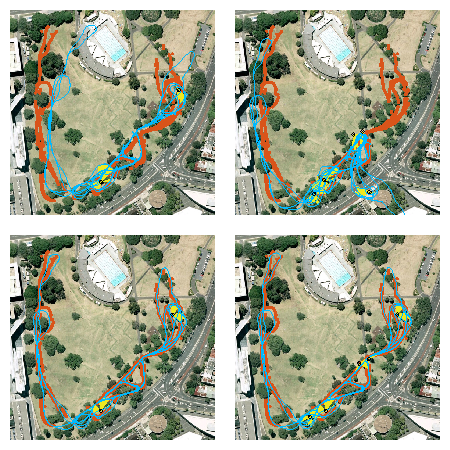
\includegraphics[width=0.48\textwidth]{fig/teaser}
  \caption{Estimating the map and trajectory (blue) on the Victoria Park dataset [4] given landmarks corrupted by simulated movement (black circle) of associated observations (yellow) and GPS ground truth (red).  (Top row) the estimation obtained by conventional graph optimization given N=2 (left) and N=5 (right) landmarks corrupted by movement. (Bottom row) the result of mobility-robust map estimation of the same data using our proposed method. Note that stationary landmarks are not shown, and GPS is unavailable at several locations.}
  \label{fig:teaser}
\end{figure}

In this paper, we present an approach to minimize the effects of
moving landmarks, by treating them as outliers, in graph-based SLAM to
improve the effectiveness of SLAM in dynamic environments.  We
propose a mobility-robustified SLAM model that includes a mobility
variable over landmarks in the joint probability to scale the effect
of a landmark in relation to how stationary it is in space.  This
mobility variable relates the belief of landmark positions with their
measurements, and diminishes moving outlier landmarks within a
measurement function (equation 4).
Effectively, this mobility variables scale the covariances
of Gaussian-distributed constraints to loosen the constrains of mobile landmarks such that their motion will push this distribution towards uniformity.
  An EM-based algorithm, as well as
an incremental version, is proposed to infer the mobility scaling
and estimate the pose trajectory of a robot with respect to a
mobility-robustified objective function. Results of our
mobility-robustified SLAM are shown respect to the
Victoria Park \cite{isam} and Alcazar of Seville \cite{iros14-frog} datasets.
